\documentclass[12pt]{article}

\usepackage[portuguese]{babel}
\usepackage{graphicx}
\usepackage{float}

\usepackage{indentfirst}

\usepackage{geometry}

\geometry{
	paper=a4paper,
	margin=60pt
}

\author{
	Felipe Scherer Vicentin\\
	248283
	\and
	Gustavo Miller Santos\\
	248320
}

\title{Diagrama de Processo}

\begin{document}

\maketitle

\section*{Visão geral do diagrama}

\begin{figure}[H]
	\centering
	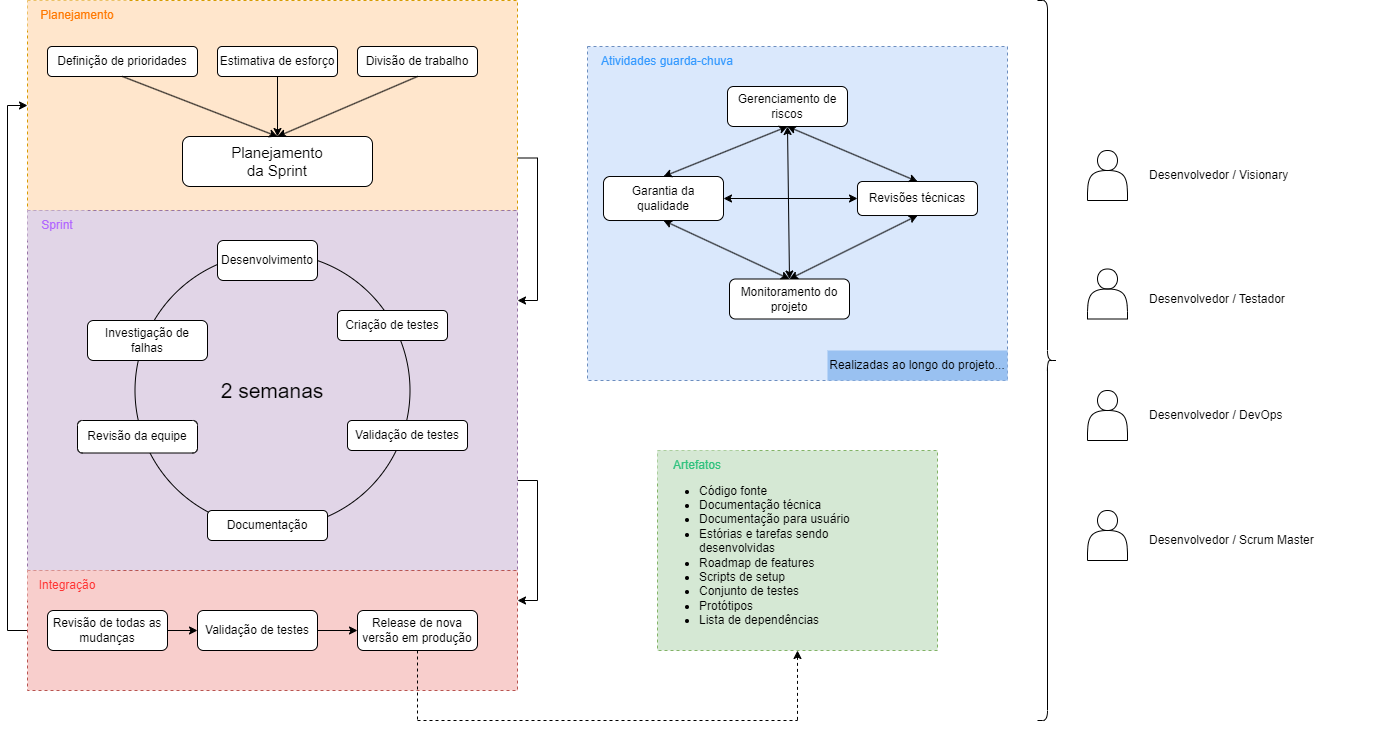
\includegraphics[width=\linewidth]{images/process_diagram.png}
\end{figure}

\section*{Explicação textual}

O processo foi dividido em planejamento, atuação cíclica (sprint), atuação constante (atividades guarda-chuva), e integração.
A ideia foi de manter um processo cíclico com iterações curtas (duas semanas), para incentivar entregas e replanejamentos frequentes.
Aqui, partimos do pressuposto que o processo seria utilizado em um projeto como o da matéria de MC426, e portanto a equipe é responsável por todas as etapas: especificação, desenvolvimento, validação e evolução.

\subsection*{Processo base}

O processo foi baseado na metodologia SCRUM:\@ iterações curtas, com uma fase de planejamento, uma de desenvolvimento, e uma de integração a cada ciclo.
Cada iteração consistirá de 2 semanas.

Similarmente ao SCRUM, o backlog é atualizado frequentemente independente dos ciclos.
No entanto, o planejamento foi simplificado para incluir o refinamento (detalhamento e estimativa de esforço), seguido de priorização, definição do que entra no ciclo seguinte, e por fim divisão de trabalho.

Feito isso, temos a sprint em si que consiste em desenvolvimento, criação e validação de testes, documentação, revisão da equipe e investigação de falhas.

Uma vez que a sprint chega ao fim, temos a etapa de integração: as mudanças são revisadas, os testes são executados, e é feita a release em produção.

\subsection*{Atividades fundamentais e guarda-chuva}

As quatro atividades fundamentais foram descritas acima. São elas:

\begin{itemize}
	\item \textbf{Especificação}: o backlog é atualizado constantemente à medida que a equipe interage para definir sua visão de longo prazo. Esse backlog é refinado na etapa de planejamento, momento em que são definidos os pormenores.
	\item \textbf{Desenvolvimento}: acontece dentro da sprint, e inclui a criação dos testes para garantia de qualidade do que foi desenvolvido.
	\item \textbf{Validação}: além dos testes, a equipe faz uma validação de cada feature a ser entregue. E ao final do ciclo, há novamente uma validação em conjunto.
	\item \textbf{Evolução}: a qualquer momento, as especificações podem ser alteradas pela equipe ou um \textit{bug} grave pode ser encontrado. Se isso acontecer, o backlog é atualizado, e as atividades serão repriorizadas para a sprint seguinte.
\end{itemize}

Já as atividades guarda-chuva, que serão feitas com frequência ao longo do projeto, incluímos:
\begin{itemize}
	\item \textbf{Gerenciamento de Riscos}: no refinamento de toda tarefa, será feita uma análise de riscos para evitar vulnerabilidades. Além disso, vulnerabilidades detectadas durante o desenvolvimento devem ser prontamente adicionadas ao backlog.
	\item \textbf{Garantia da Qualidade}: toda tarefa precisa de um critério de aceite, que deverá incluir em alto nível os testes que serão feitos para validação. Além disso, o código terá uma cobertura mínima de testes unitários, a ser definida pela equipe.
	\item \textbf{Revisões técnicas}: todo código precisa passar por uma revisão por outro membro da equipe antes de ser integrado em produção.
	\item \textbf{Monitoramento do projeto}: isso consiste em manter métricas facilmente acessíveis do projeto, que possam ser acompanhadas pela equipe. Por exemplo, cobertura de testes (monitoramento do software), disponibilidade dos recursos (monitoramento do hardware), e visibilidade do andamento das tarefas (monitoramento dos processos).
\end{itemize}

\subsection*{Principais artefatos}
\begin{itemize}
	\item \textbf{Documentação técnica}: voltada a explicar decisões sobre a arquitetura do software e detalhes de implementação.
	\item \textbf{Documentação para usuário}: guidelines de como utilizar o software desenvolvido.
	\item \textbf{Estórias e tarefas sendo desenvolvidas}: toda estória precisa ser detalhada na plataforma escolhida pela equipe (a princípio, Github Projects). Isso inclui descrição, estimativa de esforço, tarefas e critério de aceite.
	\item \textbf{Roadmap de features}: apesar de o processo ser iterativo, ainda é necessário ter uma visão macroscópica do que será entregue.
	\item \textbf{Código fonte}: inclui o código da aplicação em si, além de alguns itens como os mencionados abaixo:
	\item \textbf{Scripts de setup}: utilizados para inicializar o software desenvolvido no ambiente onde for hospedado.
	\item \textbf{Conjunto de testes}: testes unitários e de integração.
	\item \textbf{Protótipos}
	\item \textbf{Lista de dependências}
\end{itemize}


\subsection*{Papéis dos envolvidos no processo}

Como mencionado previamente, este processo seria utilizado na disciplina de MC426. Sendo assim, é ideal que todos os membros da equipe compartilhem funções, para expandir o aprendizado. Pensando nisso, definimos 4 papéis, que serão rotacionados pelos membros da equipe a cada ciclo:

\begin{itemize}
	\item \textbf{Visionary}: baseado no \textit{Dynamic System Development Method}. É a pessoa responsável por levantamento de requisitos, e a garantia de que o projeto está seguindo no caminho proposto. Não temos \textit{Ambassador User}, pois ainda não temos usuário - esse papel será feito por toda a equipe em validações.
	\item \textbf{Testador}: responsável por elaborar testes e fazer análises de qualidade do projeto.
	\item \textbf{DevOps}: responsável por garantir a integração contínua, disponibilidade dos serviços e monitoramento.
	\item \textbf{Scrum Master}: pessoa responsável por garantir que os processos estão sendo seguidos corretamente.
\end{itemize}

É importante ressaltar que essas são responsabilidades adicionais, mas todos os membros da equipe atuarão também como desenvolvedores em todos os ciclos.

\end{document}